% vim: spell spelllang=en_gb
\chapter{Methods}

This section discusses and motivates the methods used in the project. Figure~\ref{fig:flow_chart}
shows a flow chart of the steps for the pipeline (an enlarged and more detailed copy is available in
Figure~\ref{fig:flow_chart_big} of appendix \ref{appendix:raw}). The pipeline consists of the
following steps: Data collection, text classification, location extraction, text analysis, and visualization.
Python is the primary programming language used for the project because of the rich ecosystem
surrounding it, especially when it comes to data science-related tasks. The code base is available
on a GitHub
repository\footnote{https://github.com/YasserKa/Classification-and-visualization-of-natural-disasters-using-Twitter}
accompanied with a \texttt{README.md} containing instructions to set up the environment and run the
project.

\begin{figure}[H]
\begin{center}
  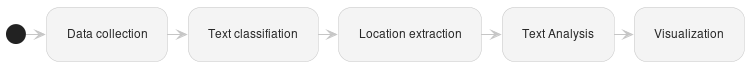
\includegraphics[width=\columnwidth]{./images/pipeline_concise.png}
\end{center}
\caption{Flow chart for the pipeline}
\label{fig:flow_chart}
\end{figure}

\section{Data Collection}

Finding a good quality data source is the first step to having a lean start for most research
questions. The pipeline trains an \ac{ML} classifier using three manually labelled datasets. Two of
them are crowdsourced datasets provided by CrisisLex6; the tweets are from the 2013 flood events in
Alberta\footnote{https://en.wikipedia.org/wiki/2013\_Alberta\_floods} and
Queensland\footnote{https://en.wikipedia.org/wiki/Cyclone\_Oswald}, and there are around 10,000
records for each one with the tweet's ID, tweet's text, and a label about the relevance of the tweet
regarding the event. The third dataset was collected and annotated in the scope of the
AI4ClimateAdaptation project and includes flood events in Sweden, spanning between 2015 and 2021; it
contains 4899 tweets, mostly in the Swedish language, with attributes presented in
Table~\ref{tab:dataset_attr}. The text and metadata of the tweets are extracted from Twitter's API
using the IDs. The trained model performance is verified using tweets extracted from the API using
Tweepy\footnote{https://docs.tweepy.org/en/latest/index.html}, a python library for accessing
Twitter API. Figure~\ref{fig:flow_chart_data_collection_text_classification} shows both the source
and usage of the data in the pipeline.

\begin{figure}[H]
\begin{center}
  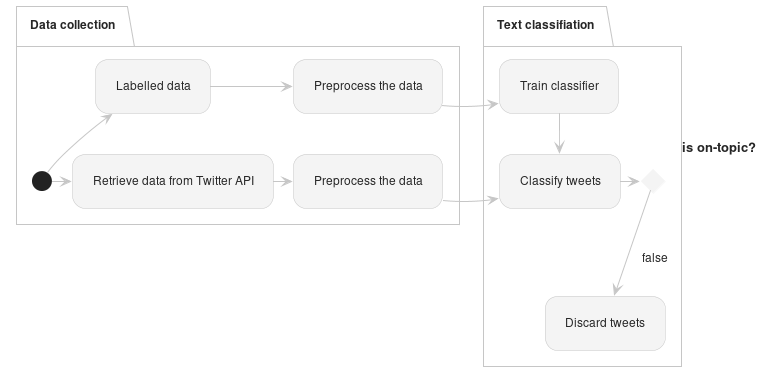
\includegraphics[width=\columnwidth]{./images/data_collection_text_classification.png}
\end{center}
\caption{Data collection and text classification steps of the pipeline}
\label{fig:flow_chart_data_collection_text_classification}
\end{figure}


\begin{table}
  \center
  \begin{tabular}{|l|l|l|}
    \hline
    Field & Type & Description \\
    \hline
    ID & Int & ID of the tweet\\
    \hline
    On Topic  & Bool & Text discusses an event \\
    \hline
    Informative sarcastic  & Bool & Text contains relevant information about the event \\
    \hline
    Contains IMPACT info & Bool & Text discusses the impact of the event \\
    \hline
    Explicit location & Bool & Text mentions the location of the event \\
    \hline
  \end{tabular}
  \caption{Dataset attributes}
  \label{tab:dataset_attr}
\end{table}

After retrieving the data, they are pre-processed to prepare them for the upcoming tasks, such as training an
\ac{ML} algorithm, text analysis, and visualization.  Parts of text that do not contribute to the
context are removed: \ac{URL}s, emojis, mentions, hashtag signs, numbers, new lines, punctuation,
and stopwords (provided by spaCy\footnote{https://spacy.io/}, an \ac{NLP} python library).
Afterwards, duplicate tweets, tweets containing no text, and retweets are discarded from the
dataset. The trained model requires the text to be in the English language, and since Sweden
is the focus of the research, most of the text is in Swedish; thus, the text is translated to
English using google translate\footnote{https://translate.google.com/} by a python library wrapper
deep-translate\footnote{https://deep-translator.readthedocs.io/en/latest/}. 

Data needs to be stored and managed to accommodate policies and regulations. Twitter's developer
policy\footnote{https://developer.twitter.com/en/developer-terms/policy} has a content
redistribution section stating that only the IDs of the tweets can be shared online. Thus, the
tweets can not be available publicly on sources, such as GitHub (the service that hosts the publicly available
code base). To this end, the data is stored after each step of the pipeline on google drive using
\ac{DVC}'s\footnote{https://dvc.org/doc} data management capabilities.


Twitter's API provides an extensive list of information about the
tweets\footnote{https://developer.twitter.com/en/docs/twitter-api/data-dictionary/object-model/tweet}.
It shares the engagement metrics of the tweet, including like count, reply count, and retweet count;
as well as, an \ac{NLP} analysis of its own, such as the language used, and entities parsed from the
text. Table~\ref{tab:tweet_attr} shows the tweet's attributes used in this project for the following reasons: the id to
generate the \ac{URL} of the tweet, the text for \ac{NLP} tasks, the created date for temporal
analysis, and the author id to reduce spam.

\begin{table}
  \center
  \begin{tabular}{|l|l|l|}
    \hline
    Attribute & Type & Description \\
    \hline
    id & Int & The unique identifier of the requested Tweet \\
    \hline
    text & Str & The actual UTF-8 text of the Tweet \\
    \hline
    created at & Date  & Creation time of the Tweet \\
    \hline
    author id & Str & The unique identifier of the tweet creator \\
    \hline
  \end{tabular}
  \caption{Tweet attributes used}
  \label{tab:tweet_attr}
\end{table}

\section{Text Classification}\label{sec:text_classification_section}

This project uses the DistilBERT transformer\cite{Sanh2019DistilBERTAD}, a variant of \ac{BERT}, for text
classification.  The main advantage of this model is that it achieves comparable performance to BERT
while being significantly smaller than BERT and more efficient. A
DistilBERT pre-trained model is provided by Hugging Face\footnote{https://huggingface.co/}, a
framework that provides a unified API for over more than 50 architectures, making it easier for
users to integrate \ac{NLP} models into their applications. The learning rate for the neural network
is $5\times e^{-5}$ with 100 warmup steps over four epochs using 90\% of the labelled tweets as
training data, 5\% as test data, and 5\% for validation. The text classification purpose is to
identify the tweets that discuss flood events, so the ``On Topic'' attribute of the dataset is used
as a label during training. 

Training the model locally takes a long time with the available resources, so the training is done
using Amazon SageMaker\footnote{https://aws.amazon.com/sagemaker/}, a service that covers tools to
build, train, and deploy \ac{ML} models. The data is uploaded to Amazon Simple Storage Service
(Amazon S3) to make it accessible for the Hugging Face training script that is executed in an
instance available in the cloud. After the training is complete, the fine-tuned model and the
evaluation metrics are downloaded. The evaluation metrics consists of the following:

\begin{itemize}
  \item Confusion matrix: a matrix showing the classifier's predictions for a labelled dataset
    corresponding to its actual values (Table~\ref{tab:confusion_matrix}).

    \begin{table}
      \center
      \bgroup
      \def\arraystretch{1.5}
      \begin{tabular}{@{}cc|cc@{}}
        \multicolumn{1}{c}{} &\multicolumn{1}{c}{} &\multicolumn{2}{c}{Predicted} \\ 
        \multicolumn{1}{c}{} & 
        \multicolumn{1}{c|}{} & 
        \multicolumn{1}{c}{Positive} & 
        \multicolumn{1}{c}{Negative} \\ 
        \cline{2-4}
        \multirow[c]{2}{*}{\rotatebox[origin=tr]{90}{Actual}}
                                     & Positive  & \ac{TP} & \ac{FN}   \\
                                     \cline{2-4}
                                     & Negative  & \ac{FP} & \ac{TN} \\
                                     \cline{2-4}
      \end{tabular}
      \egroup
      \caption{Confusion matrix}
      \label{tab:confusion_matrix}
    \end{table}

  \item Accuracy: a fraction of the number of correctly classified instances (i.e., true positives
    and true negatives) among all instances (i.e., whole dataset) (equation~\ref{eq:accuracy}).
    \begin{equation}
      \text{Accuracy}=\frac{TN+TP}{TN+FN+TP+FP} 
      \label{eq:accuracy}
    \end{equation}
  \item Precision: a fraction of the number of correctly classified relevant instances (i.e., true
    positives) among the total number of instances classified as relevant (i.e., true positives and
    false positives) (equation~\ref{eq:precision}).
    \begin{equation}
      \text{Precision}=\frac{TP}{TP+FP} 
      \label{eq:precision}
    \end{equation}
  \item Recall: a fraction of the correctly classified relevant instances (i.e., true positives)
    among all relevant instances (i.e. true positives and false negatives) (equation~\ref{eq:recall}).
    \begin{equation}
      \text{Recall}=\frac{TP}{TP+FN} 
      \label{eq:recall}
    \end{equation}
  \item $\text{F}_1$ score: a harmonic mean of precision and recall (equation~\ref{eq:f1}).
    \begin{equation}
      \text{F}_1 =2\cdot\frac{\text{Precision}\cdot\text{Recall}}{\text{Precision}+\text{Recall}} 
      \label{eq:f1}
    \end{equation}
\end{itemize}


\section{Location Extraction}

The project uses a hybrid approach for geoparsing to extract locations. For toponym recognition, the
tokens representing locations are extracted using the KBLab/bert-base-swedish-cased-ner
model\footnote{https://huggingface.co/KBLab/bert-base-swedish-cased-ner}. The model is based on BERT
and fine-tuned for \ac{NER} using The Stockholm-Umeå Corpus, a collection of Swedish texts from the
1990s that consists of one million words. As for toponym resolution, the location tokens are
disambiguated using Nominatim and GeoNames geocoders through
Geopy\footnote{https://geopy.readthedocs.io/en/latest}, a Python client for several
popular geocoding web services. Nominatim retrieves different fields about the
location from OpenStreetMap. An example of the output is available in appendix
\ref{appendix:examples}.


The descriptions for the fields are available in the
documentation\footnote{https://nominatim.org/release-docs/develop/api/Output/}. The project uses
the lat, lon, and display\_name to represent the location on a map. In some cases, the text might
contain two locations, the one with the smaller bounding box (area of corner coordinates) is used,
which is, in most cases, a more specific place located in the bigger one (e.g. a street within a
municipality). The geocoder services provide the ability to limit the search of the locations
within a specific country. Since the project is limited to Sweden, the output is limited using
this option, reducing the false positives that happen when different countries have places with
the same name. Tweets that do not contain location terms identifying a geographical
location are discarded as shown in Figure~\ref{fig:flow_chart_location_extraction}.

\begin{figure}[H]
  \begin{center}
    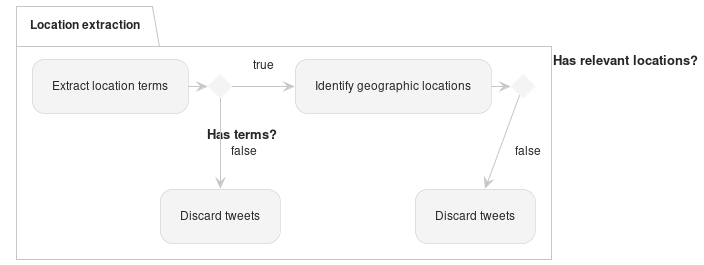
\includegraphics[width=\columnwidth]{./images/location_extraction.png}
  \end{center}
  \caption{Flow chart for the location extraction step of the pipeline}
  \label{fig:flow_chart_location_extraction}
\end{figure}


\section{Text analysis}

Further pre-processing is done on the dataset to prepare for text analysis tasks. Lemmatisation is
done on the text, using \ac{NLTK}\footnote{https://www.nltk.org/}, to reduce words to their lemmas.
Afterwards, Tokenisation is done on the corpus. Terms occurring in less than 20 documents or 5\% of
the documents are removed, as well as the terms mentioned in more than 75\% of the documents.
Bigrams that occur more than 20 times in the corpus are included, such as traffic jams, and climate
change. To reduce the impact of spambots, tweets created by the same user who tweeted about the same location the past
week are discarded.

The text analysis used in the project are \ac{LDA} \cite{pritchardInferencePopulationStructure2000}
\cite{falushInferencePopulationStructure2003}, \ac{TF-IDF}, and
\ac{t-SNE}\cite{vandermaatenVisualizingHighDimensionalData2008}. \ac{LDA} is a topic modelling
method that generates topics (a set of terms) in a corpus and assigns the relevance of each topic in
each document. Categorizing tweets can show important insights about a flood event, such as
incidents caused by floods and their impact on society. The \ac{LDA} model is initialized and
trained using Gensim \cite{rehurek_lrec}, where the number of discovered topics is adjustable in the
visualization. The second text analysis technique used is \ac{TF-IDF}, using
scikit-learn\footnote{https://scikit-learn.org/stable/}, to extract interesting terms by checking
their average weight and frequency in the corpus. Lastly, \ac{t-SNE} is a visualization method for
high-dimensional data by reducing their dimensions to two or three-dimensional maps. In this
project, \ac{t-SNE} reduces the dimensions of a \ac{TF-IDF} matrix generated from the corpus to
2-dimensional space while using the euclidean distance between tweets; afterwards, the tweets are
presented on a scatter plot with clusters generated by \ac{DBSCAN}, a density-based clustering
non-parametric algorithm. Applying dimensionality reduction on data reduces their information, so the
clustering is done before applying \ac{t-SNE} on the tweets. Presenting the tweets using a clustered
2-dimensional space makes it easier to explore tweets for insights about the discussed flood event, 
such as accidents and infrastructure damages.

\section{Visualization} 
Visualization is the final and most significant step of the pipeline since
it provides a framework for domain experts to interpret the data and gain actionable insights. Given
the nature of the problem the pipeline addresses, which is extracting information about disastrous
events, it is crucial to have several plots representing the different aspects of the events. Most
hazards impact certain regions during a time interval, so describing the spatio-temporal information
of the events is needed to analyze them. Also, since the tweets are mainly text, this allows them to
be portrayed visually after applying text analysis techniques. Another direct and beneficial use for
visualizing the data is to validate that the pipeline is functioning as intended by navigating
through the plots and checking for any suspicious results. The web application proposed in this
thesis is made by Dash\footnote{https://dash.plotly.com/} and
Plotly\footnote{https://plotly.com/python/} python packages. Dash Bootstrap
Components\footnote{https://dash-bootstrap-components.opensource.faculty.ai/} is used as well for an
easier way to use Bootstrap components for Plotly Dash, such as buttons, input, and tables.

Figure~\ref{fig:visual_interface} shows the visual interface containing all the graphs enabling
spatial, temporal, and textual exploration of the tweets: (A) a table showing tweets' properties,
(B) a map containing clusters of tweets, (C) a scatter plot for 2-dimensional representation of
tweets, (D) tables populated with terms mentioned in the tweets, and (E) a histogram for tweets'
creation dates. Users can add filtering rules for the tweets in all the plots using their creation
dates, location, and textual properties.

\begin{figure}[H]
\begin{center}
  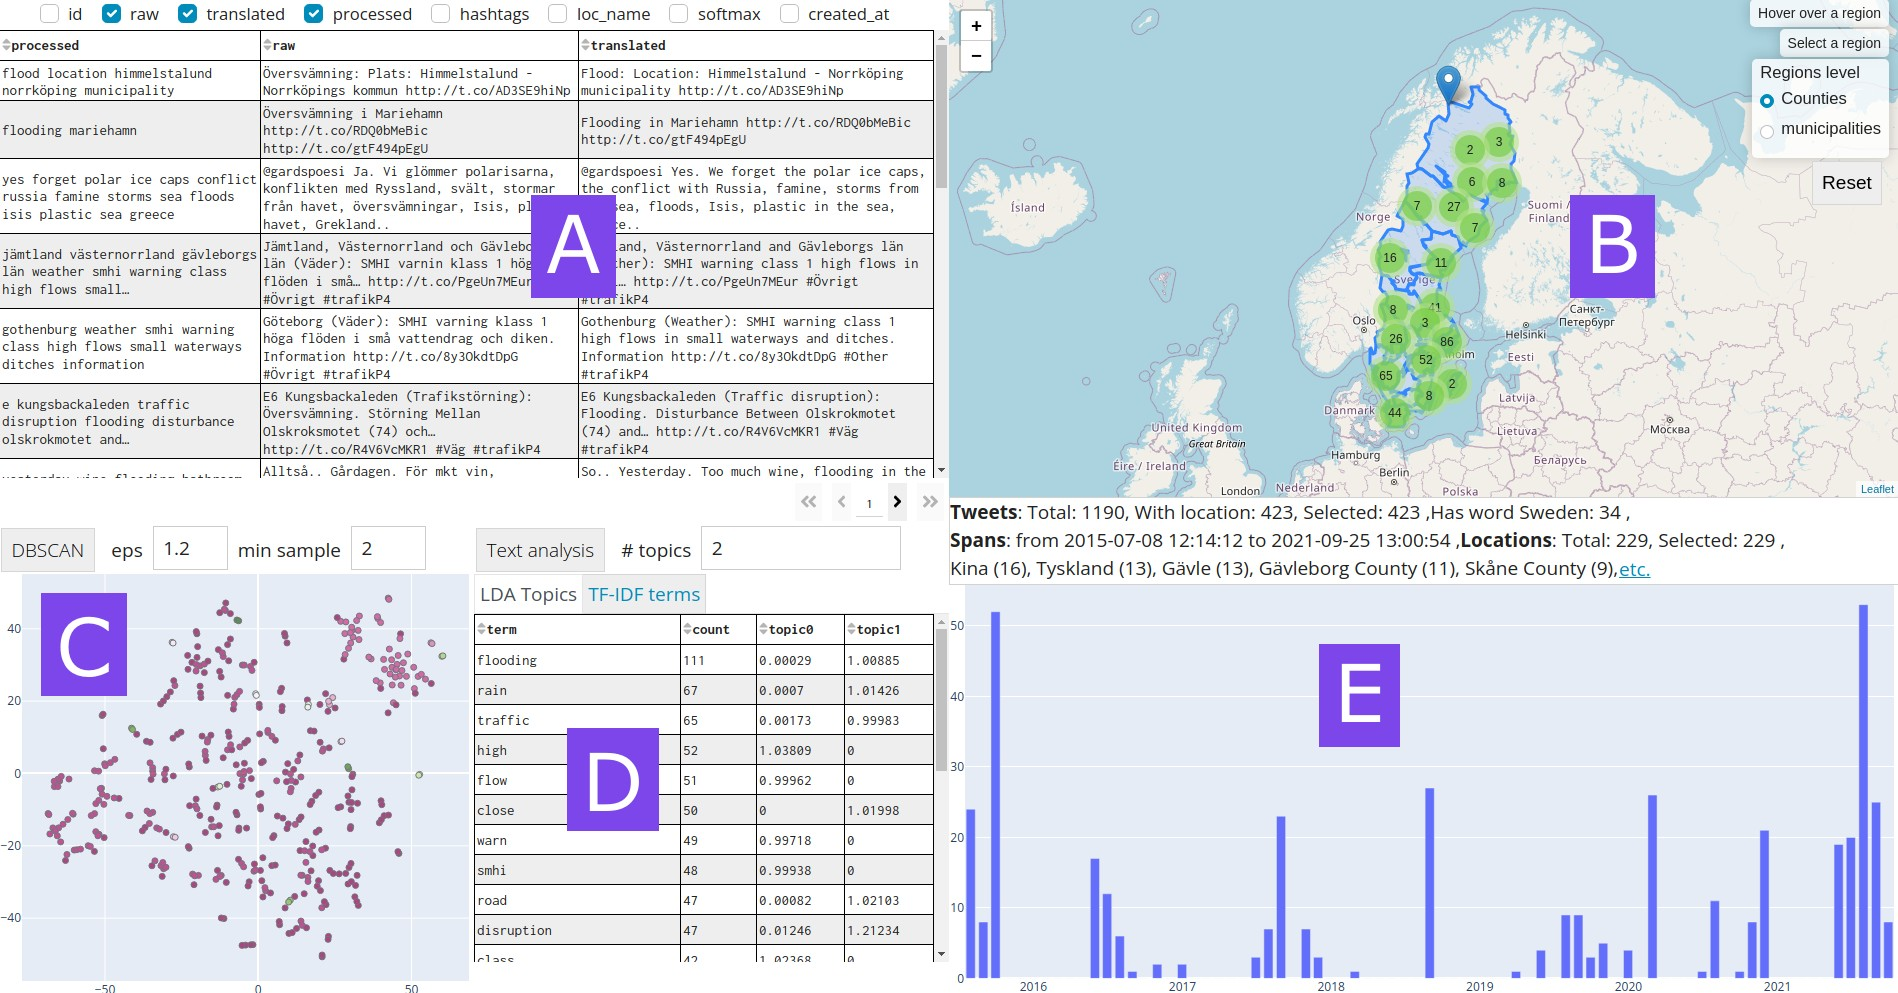
\includegraphics[width=\columnwidth]{./images/visual_interface.png}
\end{center}
\caption{The proposed visual interface with 5 plots: (A) tweets table, (B) map for extracted locations, (C)
\ac{t-SNE} scatter plot, (D) tables for \ac{LDA} and \ac{TF-IDF} terms, and (E) histogram for tweets' creation dates}
\label{fig:visual_interface}
\end{figure}

The visual interface is designed to fulfil the basic principles for the Visual Information Seeking
Mantra: ``Overview first, zoom and filter, then details-on-demand''\cite{shneidermanEyesHaveIt1996}; most of the plots
adhere to five of the seven tasks mentioned in the same paper:
\begin{itemize}
  \item Overview: Having an overview of the whole dataset.
  \item Zoom: Zooming in on an entry of interest.
  \item Filter: Disregarding uninteresting entries.
  \item Details-on-demand: Getting details on a selected entry or group when needed.
  \item Relate: Viewing the connections among entries.
\end{itemize}

The metadata in Figure~\ref{fig:meta_data}, which are displayed in the interface between the map
Fig. 3.4B and the histogram Fig. 3.4E, handles the overview task for the entire dataset. It
contains the total number of tweets, the number of selected tweets, the oldest and newest tweet
creation dates, the total number of locations, the number of selected locations, and a list of
locations' names with the number of their occurrence with an ``etc.'' button to show a pop-over
with the rest of the locations.

\begin{figure}[H]
    \begin{center}
        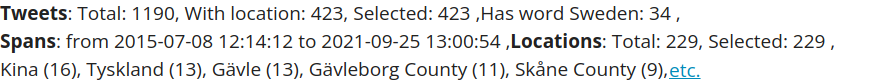
\includegraphics[width=\columnwidth]{./images/meta_data.png}
    \end{center}
    \caption{Metadata about the visual interface}
    \label{fig:meta_data}
\end{figure}


Zooming helps the users to focus on the portion of tweets they are interested in, and Plotly
supports it using the cursor for the map, histogram, and scatter plots. All plots retain the
filtering done on each one of them, so the information of the selected tweets is presented after
each filtering step, making the selected tweets easier to compare and explore; thus, satisfying the
``Details-on-demand'' and ``Relate'' tasks.

Figure~\ref{fig:map} shows the spatial distribution of tweets using an interactive map containing
clickable clustered pointers for the tweets. It makes finding locations mentioned in the tweets more
intuitive than using their toponymy. Zooming in or out disperses or congregates clusters,
respectively, providing enough clusters at any given moment. Hovering over a map pointer
shows a pop-up with the location name extracted by the pipeline. Clicking on a cluster or a region
selects the tweets they contain; this will zoom in to cover them while filtering out the unselected
pointers from the map. The top right section of the map has several elements: text elements showing
the name of the hovered and selected regions, a reset button to remove the current filter, and a
radio element to change the spatial resolution of the available regions between counties and
municipalities, enabling different granularities to filter tweets.

\begin{figure}[H]
\begin{center}
  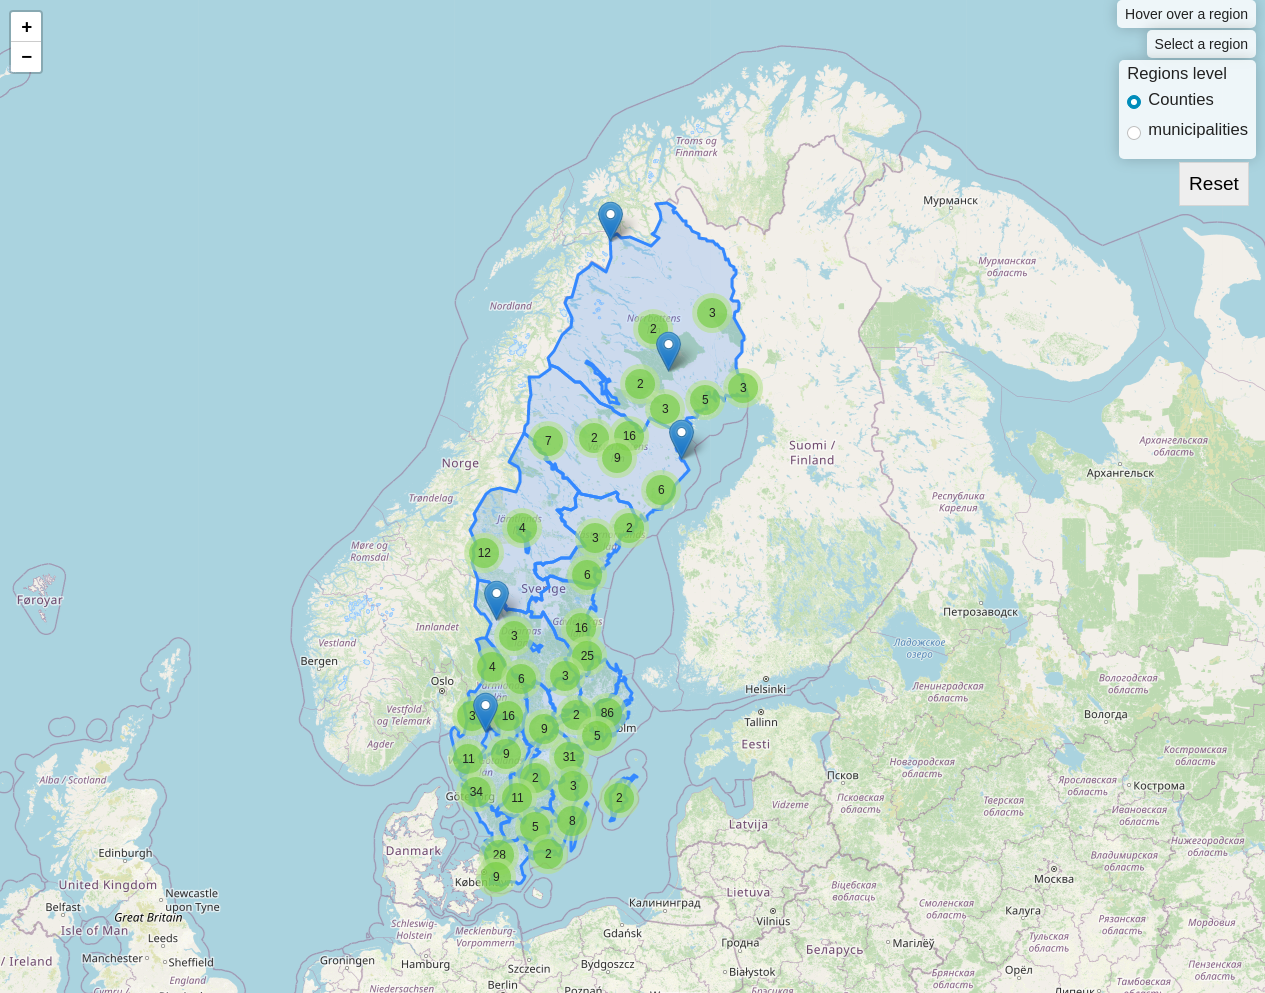
\includegraphics[width=\columnwidth]{./images/map.png}
\end{center}
\caption{Map showing clusters of tweets}
\label{fig:map}
\end{figure}

Another way to explore the tweets is by showing the temporal distribution of their creation dates
using a histogram as seen in Figure~\ref{fig:histogram}. Event detection is a good use for
histograms since they attract the attention of individuals, leading to sudden peaks that dissipate
afterwards. The dates are aggregated by day if they span a month or less; otherwise, by month.
Tweets selection is done using a select box between two dates, where the blue and red parts of the
bars represent the selected and unselected tweets, respectively. Hovering over the bars shows the
date and the number of tweets.

\begin{figure}[H]
\begin{center}
  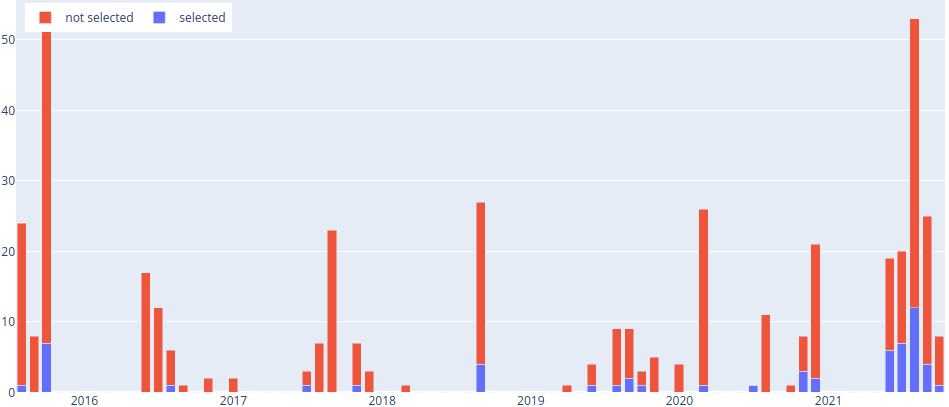
\includegraphics[width=\columnwidth]{./images/histogram.png}
\end{center}
\caption{Histogram for tweets' creation dates}
\label{fig:histogram}
\end{figure}

Tables show all the properties for data in a straightforward way to find patterns while searching
and comparing the entries among each other. The table in Figure~\ref{fig:tweets_table} shows the
selected tweets with several of their attributes: the ID, the raw (original) text, the translated
text, the processed text, the hashtags used, the location extracted, the softmax value for the
prediction, and the creation date. The table is sortable and paginated, yet it lacks the features to
satisfy the ``Filtering'' task.

\begin{figure}[H]
\begin{center}
  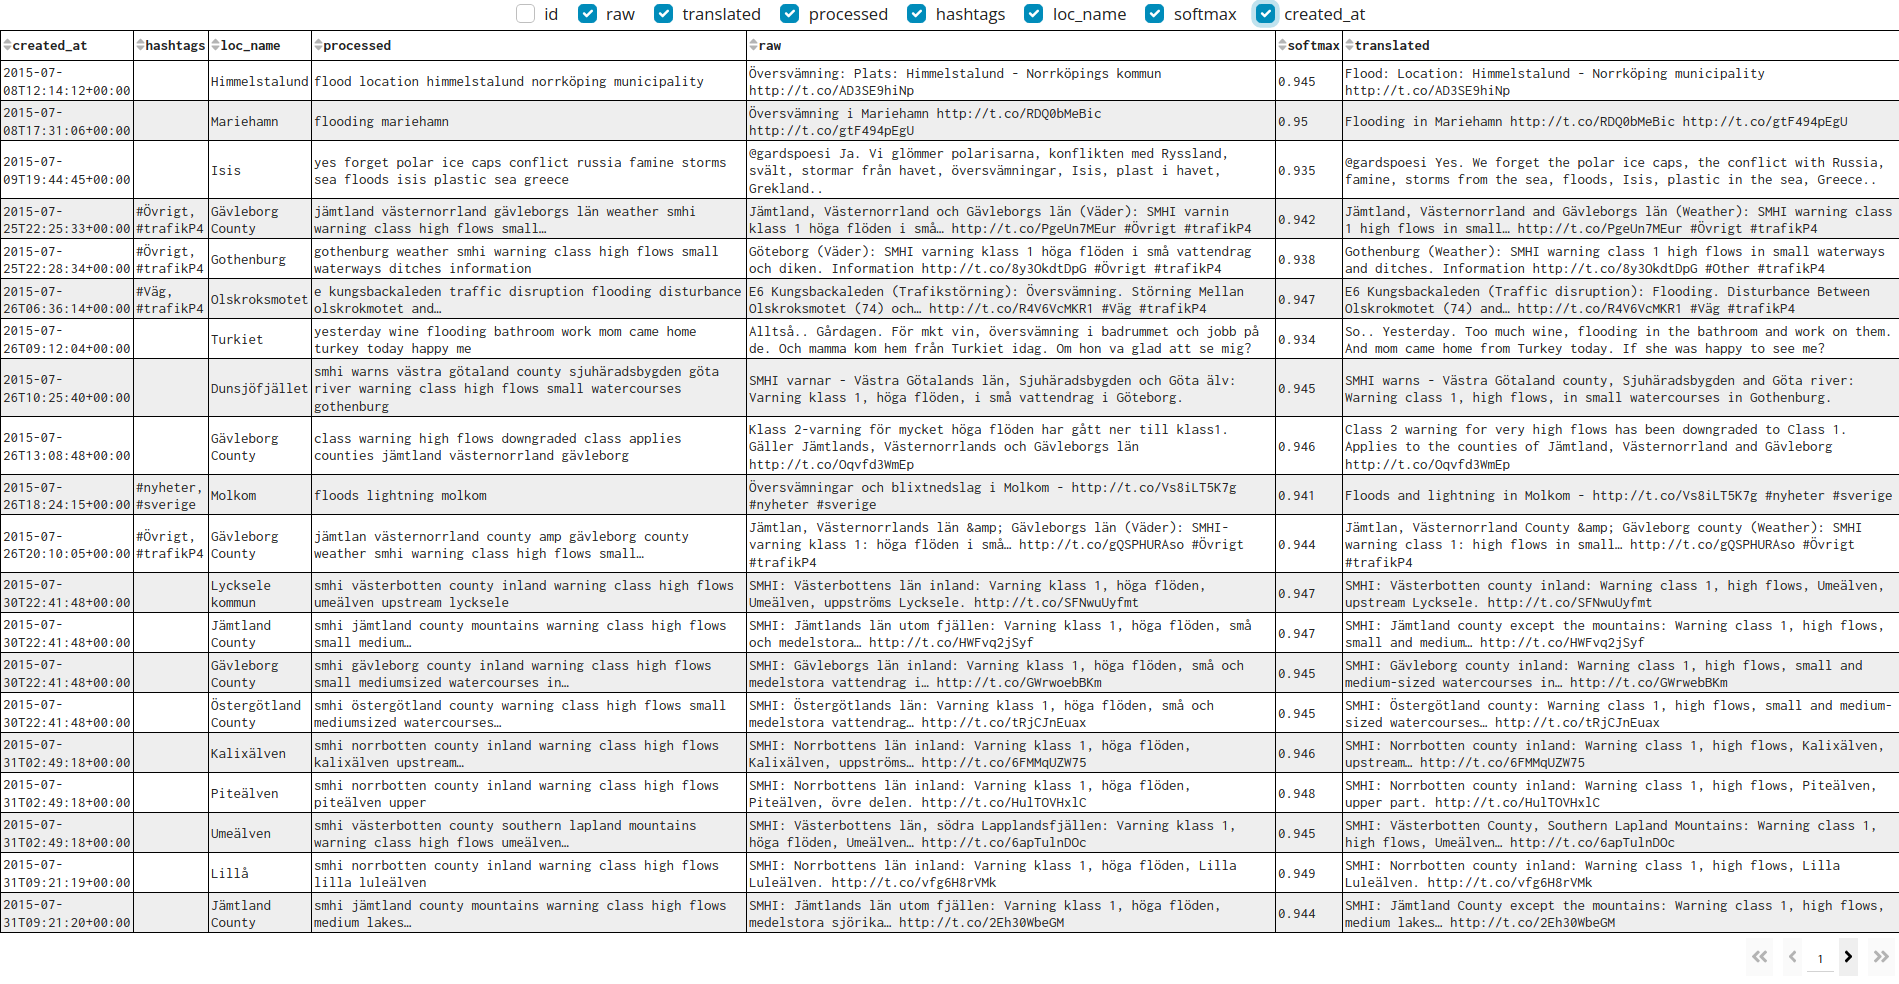
\includegraphics[width=\columnwidth]{./images/tweets_table.png}
\end{center}
\caption{Table showing the tweets}
\label{fig:tweets_table}
\end{figure}

Textual data are hard to visualize, requiring a processing step to reduce their complexity;
dimensionality reduction transforms the data from a high-dimensional space to a lower one to
represent it visually using plots. Figure~\ref{fig:scatter} shows a scatter plot for the
\ac{t-SNE}'s 2-dimensional space representation of tweets using the euclidean space with \ac{DBSCAN}
clustering, as discussed in the previous section. The clusters can be recalculated after adjusting
the properties using the text inputs above the scatter plot: ``eps'', the maximum distance between
two samples for one to be considered as in the neighbourhood of the other; and ``minimum samples'',
The number of samples (or total weight) in a neighbourhood for a point to be considered as a core
point including the point itself. Hovering over the points show a pop-up of the text for the tweets,
and the points can be selected using a box or lasso selection, meeting the ``Filtering'' task.

\begin{figure}[H]
\begin{center}
  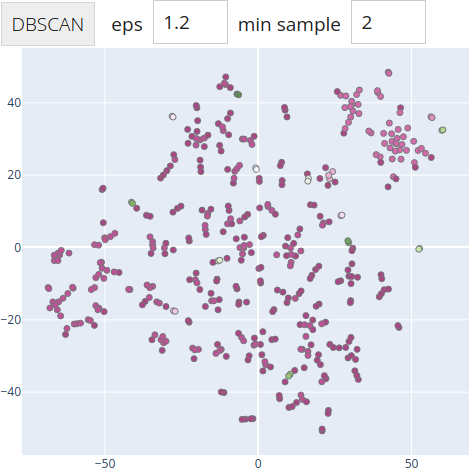
\includegraphics[width=0.5\columnwidth]{./images/scatter.png}
\end{center}
\caption{Scatter plot for \ac{t-SNE}'s space}
\label{fig:scatter}
\end{figure}

The results of \ac{LDA} and \ac{TF-IDF} are displayed in two tables (shown in
Figure~\ref{fig:lda_table} and Figure~\ref{fig:tfidf_table}, respectively)  showing the frequency of
the terms and their mean weights. The tables provide a suitable presentation to explore terms by
checking their frequency and the topics they belong to. Users can alter the number of topics
generated by \ac{LDA} using a text input and regenerate the tables on the selected tweets by
clicking the button. 

\begin{figure}[H]
    \centering
    \begin{subfigure}[b]{0.45\textwidth}
        \centering
        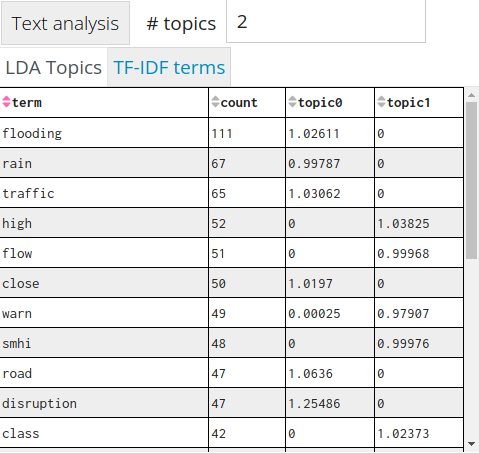
\includegraphics[width=\textwidth]{./images/lda_topics.png}
        \caption{\ac{LDA} topic weights}
        \label{fig:lda_table}
    \end{subfigure}
    \hfill
    \begin{subfigure}[b]{0.45\textwidth}
        \centering
        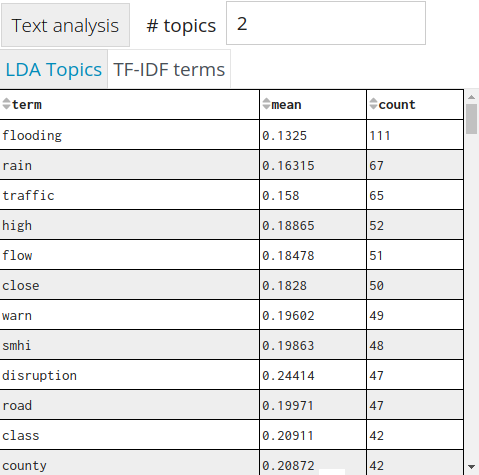
\includegraphics[width=\textwidth, trim={0 0.5cm 0 0},clip]{./images/tf_idf.png}
        \caption{\ac{TF-IDF} weights}
        \label{fig:tfidf_table}
    \end{subfigure}
    \caption{Tables showing terms with respect their frequency and their weights}
    \label{fig:tables_lda_tfidf}
\end{figure}
